%ten point, letter paper, single column
\documentclass[letterpaper,10pt, onecolumn, draftclsnofoot]{IEEEtran}

\usepackage{graphicx}                                        
\usepackage{amssymb}                                         
\usepackage{amsmath}                                         
\usepackage{amsthm}                                          

\usepackage{alltt}                                           
\usepackage{float}
\usepackage{color}
\usepackage{fancyvrb}
\usepackage{url}

\usepackage{balance}
\usepackage[TABBOTCAP, tight]{subfigure}
\usepackage{enumitem}
\usepackage{pstricks, pst-node}
\usepackage{listings}
\usepackage{tabularx}

\usepackage{geometry}
%0.75 in margin on each side, total of 1.5 in
\geometry{textheight=8.5in, textwidth=6in}

%random comment

\newcommand{\cred}[1]{{\color{red}#1}}
\newcommand{\cblue}[1]{{\color{blue}#1}}

\newcommand{\toc}{\tableofcontents}

%\usepackage{hyperref}

\def\name{Thomas Albertine}
\title{The Many Faces of Microbial Communities \\\large Senior Design\\Winter Term\\}
\author{\name, Michael Phelps}


%% The following metadata will show up in the PDF properties
% \hypersetup{
%   colorlinks = false,
%   urlcolor = black,
%   pdfauthor = {\name},
%   pdfkeywords = {capstone visualization microbiology microbio senior design},
%   pdftitle = {Senior Design Project, Visualizing Microbial Communities},
%   pdfsubject = {Senior Design Microbiology Visualizations},
%   pdfpagemode = UseNone
% }

\lstset{language=python,
                basicstyle=\ttfamily,
                keywordstyle=\color{blue}\ttfamily,
                stringstyle=\color{red}\ttfamily,
                commentstyle=\color{green}\ttfamily,
                morecomment=[l][\color{magenta}]{\#},
				breaklines=true,
				showstringspaces=false
}

\parindent = 0.0 in
\parskip = 0.1 in

%Single space
\linespread{1.0}

\usepackage{fancyvrb}
\usepackage{color}
\usepackage[latin1]{inputenc}


\makeatletter
\def\PY@reset{\let\PY@it=\relax \let\PY@bf=\relax%
    \let\PY@ul=\relax \let\PY@tc=\relax%
    \let\PY@bc=\relax \let\PY@ff=\relax}
\def\PY@tok#1{\csname PY@tok@#1\endcsname}
\def\PY@toks#1+{\ifx\relax#1\empty\else%
    \PY@tok{#1}\expandafter\PY@toks\fi}
\def\PY@do#1{\PY@bc{\PY@tc{\PY@ul{%
    \PY@it{\PY@bf{\PY@ff{#1}}}}}}}
\def\PY#1#2{\PY@reset\PY@toks#1+\relax+\PY@do{#2}}

\expandafter\def\csname PY@tok@gd\endcsname{\def\PY@tc##1{\textcolor[rgb]{0.63,0.00,0.00}{##1}}}
\expandafter\def\csname PY@tok@gu\endcsname{\let\PY@bf=\textbf\def\PY@tc##1{\textcolor[rgb]{0.50,0.00,0.50}{##1}}}
\expandafter\def\csname PY@tok@gt\endcsname{\def\PY@tc##1{\textcolor[rgb]{0.00,0.25,0.82}{##1}}}
\expandafter\def\csname PY@tok@gs\endcsname{\let\PY@bf=\textbf}
\expandafter\def\csname PY@tok@gr\endcsname{\def\PY@tc##1{\textcolor[rgb]{1.00,0.00,0.00}{##1}}}
\expandafter\def\csname PY@tok@cm\endcsname{\let\PY@it=\textit\def\PY@tc##1{\textcolor[rgb]{0.25,0.50,0.50}{##1}}}
\expandafter\def\csname PY@tok@vg\endcsname{\def\PY@tc##1{\textcolor[rgb]{0.10,0.09,0.49}{##1}}}
\expandafter\def\csname PY@tok@m\endcsname{\def\PY@tc##1{\textcolor[rgb]{0.40,0.40,0.40}{##1}}}
\expandafter\def\csname PY@tok@mh\endcsname{\def\PY@tc##1{\textcolor[rgb]{0.40,0.40,0.40}{##1}}}
\expandafter\def\csname PY@tok@go\endcsname{\def\PY@tc##1{\textcolor[rgb]{0.50,0.50,0.50}{##1}}}
\expandafter\def\csname PY@tok@ge\endcsname{\let\PY@it=\textit}
\expandafter\def\csname PY@tok@vc\endcsname{\def\PY@tc##1{\textcolor[rgb]{0.10,0.09,0.49}{##1}}}
\expandafter\def\csname PY@tok@il\endcsname{\def\PY@tc##1{\textcolor[rgb]{0.40,0.40,0.40}{##1}}}
\expandafter\def\csname PY@tok@cs\endcsname{\let\PY@it=\textit\def\PY@tc##1{\textcolor[rgb]{0.25,0.50,0.50}{##1}}}
\expandafter\def\csname PY@tok@cp\endcsname{\def\PY@tc##1{\textcolor[rgb]{0.74,0.48,0.00}{##1}}}
\expandafter\def\csname PY@tok@gi\endcsname{\def\PY@tc##1{\textcolor[rgb]{0.00,0.63,0.00}{##1}}}
\expandafter\def\csname PY@tok@gh\endcsname{\let\PY@bf=\textbf\def\PY@tc##1{\textcolor[rgb]{0.00,0.00,0.50}{##1}}}
\expandafter\def\csname PY@tok@ni\endcsname{\let\PY@bf=\textbf\def\PY@tc##1{\textcolor[rgb]{0.60,0.60,0.60}{##1}}}
\expandafter\def\csname PY@tok@nl\endcsname{\def\PY@tc##1{\textcolor[rgb]{0.63,0.63,0.00}{##1}}}
\expandafter\def\csname PY@tok@nn\endcsname{\let\PY@bf=\textbf\def\PY@tc##1{\textcolor[rgb]{0.00,0.00,1.00}{##1}}}
\expandafter\def\csname PY@tok@no\endcsname{\def\PY@tc##1{\textcolor[rgb]{0.53,0.00,0.00}{##1}}}
\expandafter\def\csname PY@tok@na\endcsname{\def\PY@tc##1{\textcolor[rgb]{0.49,0.56,0.16}{##1}}}
\expandafter\def\csname PY@tok@nb\endcsname{\def\PY@tc##1{\textcolor[rgb]{0.00,0.50,0.00}{##1}}}
\expandafter\def\csname PY@tok@nc\endcsname{\let\PY@bf=\textbf\def\PY@tc##1{\textcolor[rgb]{0.00,0.00,1.00}{##1}}}
\expandafter\def\csname PY@tok@nd\endcsname{\def\PY@tc##1{\textcolor[rgb]{0.67,0.13,1.00}{##1}}}
\expandafter\def\csname PY@tok@ne\endcsname{\let\PY@bf=\textbf\def\PY@tc##1{\textcolor[rgb]{0.82,0.25,0.23}{##1}}}
\expandafter\def\csname PY@tok@nf\endcsname{\def\PY@tc##1{\textcolor[rgb]{0.00,0.00,1.00}{##1}}}
\expandafter\def\csname PY@tok@si\endcsname{\let\PY@bf=\textbf\def\PY@tc##1{\textcolor[rgb]{0.73,0.40,0.53}{##1}}}
\expandafter\def\csname PY@tok@s2\endcsname{\def\PY@tc##1{\textcolor[rgb]{0.73,0.13,0.13}{##1}}}
\expandafter\def\csname PY@tok@vi\endcsname{\def\PY@tc##1{\textcolor[rgb]{0.10,0.09,0.49}{##1}}}
\expandafter\def\csname PY@tok@nt\endcsname{\let\PY@bf=\textbf\def\PY@tc##1{\textcolor[rgb]{0.00,0.50,0.00}{##1}}}
\expandafter\def\csname PY@tok@nv\endcsname{\def\PY@tc##1{\textcolor[rgb]{0.10,0.09,0.49}{##1}}}
\expandafter\def\csname PY@tok@s1\endcsname{\def\PY@tc##1{\textcolor[rgb]{0.73,0.13,0.13}{##1}}}
\expandafter\def\csname PY@tok@sh\endcsname{\def\PY@tc##1{\textcolor[rgb]{0.73,0.13,0.13}{##1}}}
\expandafter\def\csname PY@tok@sc\endcsname{\def\PY@tc##1{\textcolor[rgb]{0.73,0.13,0.13}{##1}}}
\expandafter\def\csname PY@tok@sx\endcsname{\def\PY@tc##1{\textcolor[rgb]{0.00,0.50,0.00}{##1}}}
\expandafter\def\csname PY@tok@bp\endcsname{\def\PY@tc##1{\textcolor[rgb]{0.00,0.50,0.00}{##1}}}
\expandafter\def\csname PY@tok@c1\endcsname{\let\PY@it=\textit\def\PY@tc##1{\textcolor[rgb]{0.25,0.50,0.50}{##1}}}
\expandafter\def\csname PY@tok@kc\endcsname{\let\PY@bf=\textbf\def\PY@tc##1{\textcolor[rgb]{0.00,0.50,0.00}{##1}}}
\expandafter\def\csname PY@tok@c\endcsname{\let\PY@it=\textit\def\PY@tc##1{\textcolor[rgb]{0.25,0.50,0.50}{##1}}}
\expandafter\def\csname PY@tok@mf\endcsname{\def\PY@tc##1{\textcolor[rgb]{0.40,0.40,0.40}{##1}}}
\expandafter\def\csname PY@tok@err\endcsname{\def\PY@bc##1{\setlength{\fboxsep}{0pt}\fcolorbox[rgb]{1.00,0.00,0.00}{1,1,1}{\strut ##1}}}
\expandafter\def\csname PY@tok@kd\endcsname{\let\PY@bf=\textbf\def\PY@tc##1{\textcolor[rgb]{0.00,0.50,0.00}{##1}}}
\expandafter\def\csname PY@tok@ss\endcsname{\def\PY@tc##1{\textcolor[rgb]{0.10,0.09,0.49}{##1}}}
\expandafter\def\csname PY@tok@sr\endcsname{\def\PY@tc##1{\textcolor[rgb]{0.73,0.40,0.53}{##1}}}
\expandafter\def\csname PY@tok@mo\endcsname{\def\PY@tc##1{\textcolor[rgb]{0.40,0.40,0.40}{##1}}}
\expandafter\def\csname PY@tok@kn\endcsname{\let\PY@bf=\textbf\def\PY@tc##1{\textcolor[rgb]{0.00,0.50,0.00}{##1}}}
\expandafter\def\csname PY@tok@mi\endcsname{\def\PY@tc##1{\textcolor[rgb]{0.40,0.40,0.40}{##1}}}
\expandafter\def\csname PY@tok@gp\endcsname{\let\PY@bf=\textbf\def\PY@tc##1{\textcolor[rgb]{0.00,0.00,0.50}{##1}}}
\expandafter\def\csname PY@tok@o\endcsname{\def\PY@tc##1{\textcolor[rgb]{0.40,0.40,0.40}{##1}}}
\expandafter\def\csname PY@tok@kr\endcsname{\let\PY@bf=\textbf\def\PY@tc##1{\textcolor[rgb]{0.00,0.50,0.00}{##1}}}
\expandafter\def\csname PY@tok@s\endcsname{\def\PY@tc##1{\textcolor[rgb]{0.73,0.13,0.13}{##1}}}
\expandafter\def\csname PY@tok@kp\endcsname{\def\PY@tc##1{\textcolor[rgb]{0.00,0.50,0.00}{##1}}}
\expandafter\def\csname PY@tok@w\endcsname{\def\PY@tc##1{\textcolor[rgb]{0.73,0.73,0.73}{##1}}}
\expandafter\def\csname PY@tok@kt\endcsname{\def\PY@tc##1{\textcolor[rgb]{0.69,0.00,0.25}{##1}}}
\expandafter\def\csname PY@tok@ow\endcsname{\let\PY@bf=\textbf\def\PY@tc##1{\textcolor[rgb]{0.67,0.13,1.00}{##1}}}
\expandafter\def\csname PY@tok@sb\endcsname{\def\PY@tc##1{\textcolor[rgb]{0.73,0.13,0.13}{##1}}}
\expandafter\def\csname PY@tok@k\endcsname{\let\PY@bf=\textbf\def\PY@tc##1{\textcolor[rgb]{0.00,0.50,0.00}{##1}}}
\expandafter\def\csname PY@tok@se\endcsname{\let\PY@bf=\textbf\def\PY@tc##1{\textcolor[rgb]{0.73,0.40,0.13}{##1}}}
\expandafter\def\csname PY@tok@sd\endcsname{\let\PY@it=\textit\def\PY@tc##1{\textcolor[rgb]{0.73,0.13,0.13}{##1}}}

\def\PYZbs{\char`\\}
\def\PYZus{\char`\_}
\def\PYZob{\char`\{}
\def\PYZcb{\char`\}}
\def\PYZca{\char`\^}
\def\PYZam{\char`\&}
\def\PYZlt{\char`\<}
\def\PYZgt{\char`\>}
\def\PYZsh{\char`\#}
\def\PYZpc{\char`\%}
\def\PYZdl{\char`\$}
\def\PYZti{\char`\~}
% for compatibility with earlier versions
\def\PYZat{@}
\def\PYZlb{[}
\def\PYZrb{]}
\makeatother


\begin{document}
\maketitle
\section*{Abstract}
We intend for this project to provide an easier to use way to visualize microbial population data than some existing techniques, such as pie or bar charts, within the constraints provided by our client. As of the midterm progress report, we have had working backend components for loading population data files in the QIIME OTU format, generating 3d models based on the data in Wavefront obj format, and converting population counts into normalized values that can be used to generate 3D models of human faces, as well as a preliminary user interface (UI) for most of our project. Since then, we've improved the UI, connected the UI with backend functionality mentioned before, and done user testing to identify new improvements to be made. The remaining work is simply to fix the problems we've identified in our testing, continue testing to identify more problems, and possibly implement some of our stretch goals, such as expanding file format support.

\clearpage

\tableofcontents

\section{A Note Regarding Division of Labor in this Document and the Corresponding Video}
During the midterm progress report, we split the work, such that Thomas primarily worked on the written report, and Michael primarily worked on the video. This was because Thomas had a cold and did not want to be in the video. However, we feel that dividing the work in this way allowed us to provide a better result than we would have otherwise, with a few exceptions due to poor communication.

For this report, we intend to do something similar, but with more thorough proofreading after the rough draft is complete. Therefore, Thomas will again not be appearing in the video, and will focus on the report instead. Unlike before however, Thomas will send Michael his notes on the video, and Michael will send Thomas his notes on this document, which should cut back on mistakes in both.

\section{Purposes and Goals}

The purpose of the project is to visualize microbial population data in a way that allows microbiologists (and secondarily other researchers) to more easily compare complex population data. To that effect, our client has requested that we model it as human-esque faces, in order to take advantage of humans' ability to recognize and compare those faces. Resulting models need not look like visually appealing humans, but they should represent the data.

To that effect, our project loads population data from files in supported formats and sample grouping data in corresponding metadata files. This data is converted to model attributes, values that determine how exaggerated some feature of the face, called a model parameter, is, based on associations provided by the user in the application. These attributes are passed into MakeHuman, an open source project that generates 3d models of humans. It generates 3D models in Wavefront obj format for each sample. Then the models are then loaded and displayed to the user, who can view smaller sets of samples based on grouping data, or can choose a subset of no more than six samples to view and inspect in more detail.

\section{Completed Content}

\subsection{Backend}

\begin{figure}
	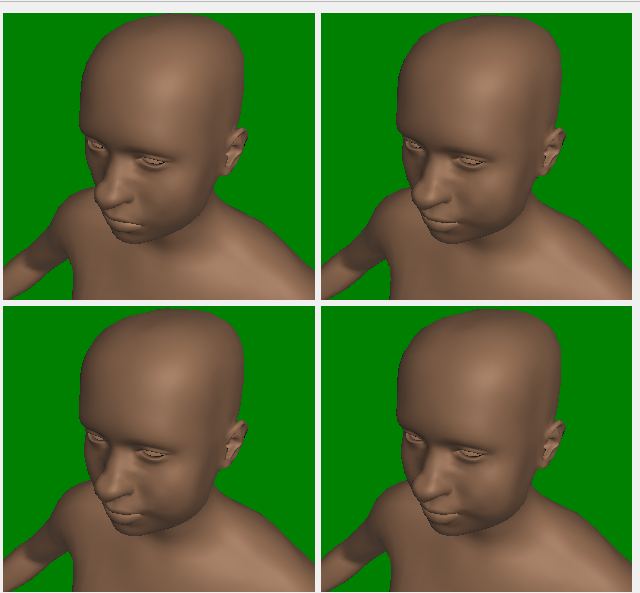
\includegraphics[width=\textwidth]{analysis}
	\caption{A model generated from a sample data file. This file had few enough organisms that only some features were modified. The rest were left at their default values to avoid distracting from the significant features of the data set. This image was generated using an obj viewer widget that Thomas wrote and the analysis view page that Michael wrote.}
	\label{fig:generated}
\end{figure}

In the backend code of the project, Thomas has already written a wrapper around MakeHuman that can retrieve a list of valid model parameter names\footnote{Our requirements document specifies that we support 150 model parameters, but we only have enough facial features to support 138. We can extend that number significantly however, if we use other model parameters besides facial features, but our client mainly wants to work with facial features alone. We are considering adding the others as optional parameters.} as well as receive model parameter names and values in order to generate models. This particular code has a minor deficiency in that the models it produces have no eyes, so if we have time to improve upon it later, we intend to. That said, if it proves impossible, the current system is still sufficient to visualize the data. Figure \ref{fig:generated} depicts a model generated from a data file.

Thomas\footnote{Originally, Michael started writing this component, but there was a miscommunication and Thomas panicked and wrote it instead.} has also written code to load a QIIME OTU tab-delineated data file, which the client specified as the minimum for data loading, as well as a framework to allow us to easily add support for other file types later on. This is described in more detail in section \ref{interestingCode} later in this document, but in short, we create a python object that can parse a file format, and associate it with certain file extensions in a registry object that we have also created. When loading a file, simply pass the file path into the registry object, and it uses the extension from the file path to find the right parser, which is passed the file path. Each parser object is responsible for parsing the data file itself, as well as the metadata file that contains grouping information.

Thomas has also written code to normalize sample data based on the largest population in the sample (in order to compare ratios of populations between samples), based on the largest population in the file (in order to compare population sizes between samples), and based on a manual scaling value that can be set by the user, in order to compare between images of previously generated models, or models in separate files.

\subsection{Frontend}

Michael has written the data loading page, the main selection page, and the detailed viewing page. Currently, the grouping functionality, model generation, and microbe-model parameter mapping, are all connected to the UI

Thomas has written an obj viewer widget that Michael is using to display the obj files.

\begin{figure}
	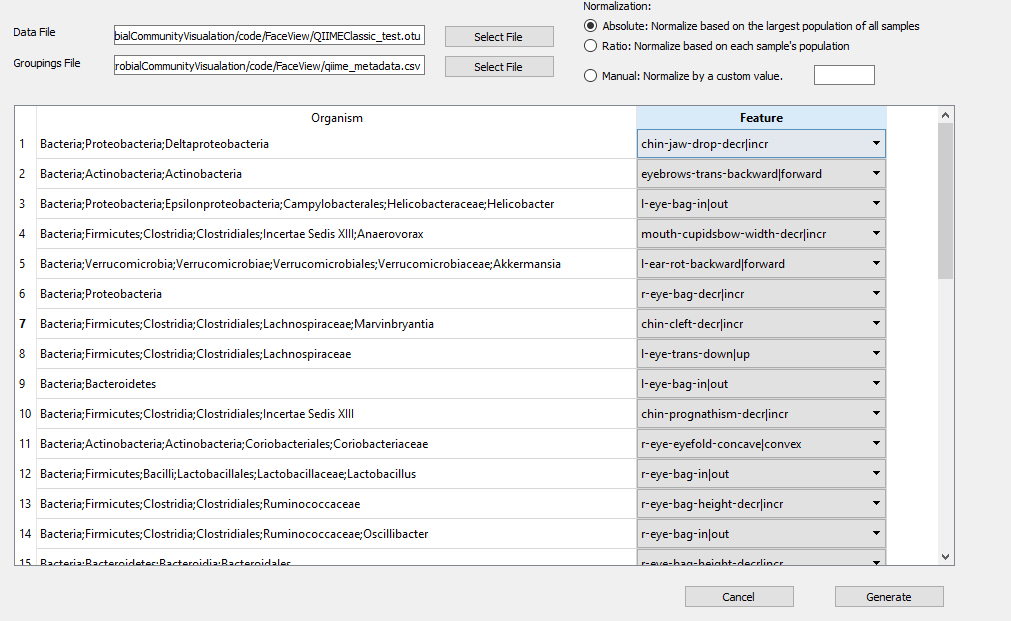
\includegraphics[width=\textwidth]{loading}
	\caption{The UI page that allows users to perform tasks related to loading data files.}
	\label{fig:LoadingInterface}
\end{figure}

The Data Loading page (see Figure \ref{fig:LoadingInterface}) allows users to select a data file and a groupings file. These files will be loaded, and then used to populate the table on the bottom, which allows users to associate model parameters with organisms in the sample. On the top right, a series of radio buttons can be used to specify which normalizing strategy to use. That is, whether the generated models should reflect ratio of each organism to the whole of the sample, or whether the generated models should reflect the ratio of each organism to the largest population in the file, or whether the models should be normalized in terms of some other number entirely. The first is good for identifying samples with similar ratios of an organism to the population in the sample. The second is good for identifying samples with similar total populations of an organism. The third is good for comparing models in a different file.

\begin{figure}
	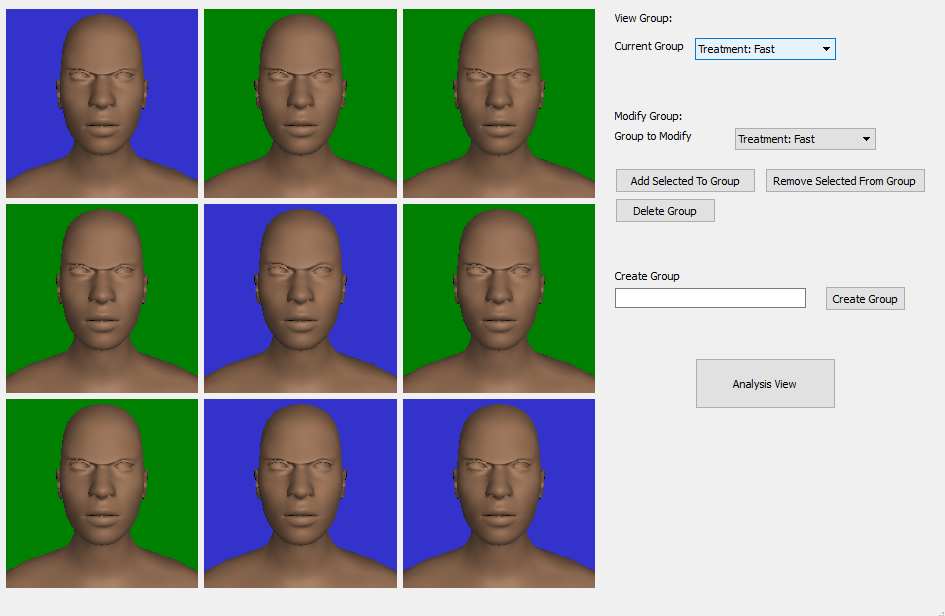
\includegraphics[width=\textwidth]{Comparison}
	\caption{The UI page that allows users to perform tasks related to selecting data files.}
	\label{fig:MainInterface}
\end{figure}

The Main Selection page (see Figure \ref{fig:MainInterface}) will allow users to select a few samples out of the file to examine in more detail. The box on the left is where images of the samples' models will appear, while the elements on the right allow users to organism samples into groups, or view groups from the metadata file.

\section{Remaining Work}\label{rWork}

There still exist some notable bugs. Specifically, once the user goes forward to a new page, he or she cannot go back at this time. When the user opens the analysis view, the thumbnail view does not close, but becomes unresponsive, which could lead to confusion for users. Finally, when the application is closed, Windows displays an error message that python is not responding, which does not directly inhibit usability, but should still be fixed before release.

Additionally, our user testing has revealed several opportunities for improvement that we'd like to implement. One of our test subjects suggested that the blue and green backgrounds in the thumbnail view which denote whether the sample is selected or not are not intuitive, and that we should use different colors. More than one of our subjects suggested that the model parameters are difficult to understand. We believe that we can resolve this by adding a system to alias the model parameters taken directly from MakeHuman to something more easily understood. Another test subject pointed out that the images of the models are not drawn with the names of their corresponding samples, which could significantly improve usability, but should be easily fixed. Test subjects would also click the model generator button multiple times because there was no cue for them to know that the first click had done something. We'd like to either add something to the window to show that, or close that window to reveal the console so that the user knows that the application is making progress. Finally, our last subject suggested that not every model parameter is visible from the front view provided by thumbnail view. We think that this could be resolved by turning the models back and forth slowly.

When these issues are resolved at least, then we will consider version 1.0 complete, although if we have time to implement any of our stretch goals too, so be it.

As mentioned in the backend section, if time allows, we would also fix the eye problem with model generation and improve our testing.



\section{Significant Problems and Associated Solutions}

The most difficult problem that Thomas faced was simply trying to read and decypher the MakeHuman code enough to write the wrapper. Since Python is loosely typed, he couldn't just match the types to see how things were being used. Instead (at least at first), he had to walk through the code jumping from function definition to function definition, searching through multiple files. After doing that for a few hours, he remembered that python objects have a dictionary of their attributes, so he was able to import MakeHuman modules and examine the the contents of objects returned from functions. This sped up the process considerably. Additionally, he figured out how to use grep-like functionality from within PowerShell, which made it much easier to look for function definitions.

Additionally, the obj viewer widget proved challenging simply because the the error policy for OpenGL is to fail silently and not draw anything. Most of this can be mitigated by occasional calls to $glGetError()$, but some mistakes are not technically errors, yet still don't produce the intended output.

For Michael, the most difficult problem was figuring out how to display the obj files within the Qt based interface. There is surprisingly little documentation on how to perform such a task. As of now, the obj viewer widget should solve these problems, but nevertheless, it was a concern earlier on, and one that Michael put an exceptional amount of work into.

\section{Interesting Code} \label{interestingCode}

\subsection{fvParser} 

The following is the framework for easy addition of new parsers. minParser represents the minimum functionality required for a parser. If this were C++, it would be a virtual class, but thanks to Python's duck typing, we don't actually have to inherit from anything, so it's more of a template for us to copy later.

The ParserRegistry itself is little more than a wrapper around a dictionary, mapping a file extension to a parser object, but with some additional functions added to it to make its usage more obvious. Finally, an instance of the Registry is created as a global, so that it can be referenced anywhere by importing the module.

\lstinputlisting[language=python]{../../code/FaceView/fvParser.py}

\subsection{objWidget} 

The following is a PyQt widget written by Thomas which inherits from the QOpenGLWidget in standard PyQt. Additionally, the file includes additional functions used by the class for creating transformation and projection matrices. The class itself accepts a 3d model object

\lstinputlisting[language=python]{../../code/FaceView/objViewer/objWindow.py}

\section{User Study}

We have completed our first user study and gained some suggestions and insight to improve the project's usability. 

\subsection{Users}

For our test subjects, we found college students of various disciplines and backgrounds. This was more than sufficient to provide suggestions about, and identify flaws in, our UI, especially since it is relatively new and untested.

\subsection{Methods}

We used a set of 5 moderated, in-person tests. This was enough to identify several bugs and other opportunities for improvement, but not so many that it took an impractical amount of time to moderate it.

\subsection{Tasks}

Before each task, we asked users how confident they are that they can complete the task, and timed them while they performed the task, recording the time it took them. When we saw them struggling over a particular step in the task, we made a note of it. If the user seemed unable to make progress, we made a note of what step they were stuck on, politely interrupted them, and completed the step ourselves so that the user could see how it was done. When users requested that we repeat the task statement or some detail of it, we did. None requested clarification, but if they had, we would answer their questions and make a note of that as well, so that we could design a better test in the future.

Our tasks are as follows, starting immediately after opening the application for the first time, and given a sample data file:
\begin{enumerate}
	\item Load the data file.
	\item Associate Bacillus subtilis with head squareness\footnote{This organism and this model parameter need not be the ones used in the test}.
	\item Modify settings so that you can compare ratios of different populations between samples.
	\item Generate the models.
	\item Select some samples to compare in more detail.
	\item Find the two samples with the most similar ratios of Bacillus subtilis to total population and view them in more detail.
	\item Find the two samples with the most similar total population of bacillus subtilis and view them in more detail.
\end{enumerate}

After the first few tests, we removed a task ``Manipulate Models'' because users invariably started playing with that feature before we had a chance to time them or ask them anything about it.

The first five tasks are primarily to identify how intuitive the application is to a new user. The last two are to identify how easy the application is to use once someone has seen how it works.

\subsection{Results}

From our testing, we were able to better understand which areas of our UI needed the most improvement. These improvements are described in section \ref{rWork}, Remaining Work.

\begin{figure}
\begin{tabularx}{\textwidth}{|X|X|X|X|X|X|X|}
\hline
Task & \multicolumn{6}{X|}{Subject} \\
\cline{2-7}
& 1 & 2 & 3 & 4 & 5 & Average Time \\
\hline
1    & ``Yes'' 0:31 & ``Yes'' 0:44        & ``Medium'' 0:20         & ``In the middle'' 0:56 & ``Yes'' 0:38 & 0:38 \\
\hline
2    & ``No'' 1:00  & ``Don't Know'' 0:12 & ``Very Confident'' 0:01 & ``Medium'' 2:00        & ``No'' 0:11  & 0:41 \\
\hline
3    & ``Yes'' 0:02 & ``Yes'' 0:03        & ``Confident'' 0:01      & ``4/10'' 2:27          & ``No'' 0:22  & 0:35 \\
\hline
4    & ``Yes'' 0:10 & ``Yes'' 0:12        & ``Confident'' 0:10      & ``4/10'' 0:10          & ``Yes'' 0:10 & 0:10 \\
\hline
5    & ``No'' 1:20  & ``No'' 0:09         & ``Confident'' 1:00      & ``5/10'' 0:09          & ``No'' 0:11  & 0:34 \\
\hline
6    & ``Yes'' 1:26 & ``Yes'' 0:53        & ``Maybe'' 3:03          & ``6/10'' 3:08          & ``No'' 0:59  & 1:54 \\
\hline
7    & ``Yes'' 0:57 & ``Yes'' 1:27        & ``Yes'' 0:50            & ``Yes'' 1:40           & ``Yes'' 1:54 & 1:22 \\
\hline

\end{tabularx}
\caption{This is the data from our UI testing. The middle cells contains the user's description of his or her confidence before attempting each task as well as the time it took the user to complete the task}
\label{fig:uiTestData1}
\end{figure}

Figure \ref{fig:uiTestData1} contains our data for the ui testing. In addition, we also have a series of observations that we made while watching our subjects, and comments that our subjects made when we asked them afterwards.

\subsubsection{Subject 1}
This subject is a junior majoring in biology. During task 5, she found that the blue and green colors we currently use to denote whether the models are not particularly intuitive. During task 6, she spent longer than expected looking through the model parameter options than we expected, which delayed her completion time. Afterwards, she commented that the names in the model parameter dropdown were not particularly intuitive.

\subsubsection{Subject 2}
This subject is a freshman majoring in his mechanical engineering, and who's first language is not English. He discovered that not every selected sample appears in the analysis page when the analysis view button is clicked, a bug that has since been fixed. He also commented that the model parameter list is ``detailed'', and that the samples do not show their sample name in the thumbnail view.

\subsubsection{Subject 3}
This subject is a freshman majoring in computer science. He showed signs of being competitive regarding completion times, but got distracted looking through the model parameter list, which delayed his completion time. He commented that he was confused about how the data sets corresponded to the generated faces, but later said that the relationship was intuitive if the user understands what the input data contains.

\subsubsection{Subject 4}
This subject is a college freshman majoring in business. He showed signs of being tired or not having slept enough recently, which may have affected his results. He made jokes about sleep deprived researchers which seems to confirm my observation. Initially, the subject had difficulty using functionality provided by Windows, accidentally minimizing the window, and then closing it while trying to unminimize it, but he did better once we reopened it for him. 

During task 2, he commented that the tool was ``very thorough''. During task 3, he was unable to find the radio button that specifies that data be normalized as a percentage of the total sample population, requiring me to point it out to him. During task 4, while waiting for the models to generate, he suggested adding something to let the user know that the application is making progress.

Afterwards, the subject said that the tasks were difficult and that he would like to try again for a shorter completion time. He also mentioned that the relationship between the model parameters and their effect on the generated model was not particularly intuitive.

\subsubsection{Subject 5}
This subject is a college senior majoring in fish and wildlife who claims to be bad with computers. During task 7, he mentioned that not all model features are visible from the front view provided from the thumbnail view page, and suggested making the models rotate.

\end{document}
